\documentclass{beamer}
\usetheme{default}
\usecolortheme{default}
\setbeamertemplate{navigation symbols}{}
\setbeamertemplate{footline}[frame number]

\usepackage{amsmath,amssymb,amsthm}
\usepackage{graphicx}
\usepackage{booktabs}
\usepackage{algorithm}
\usepackage{algpseudocode}
\usepackage{xcolor}
\usepackage{float}
\usepackage{tikz}
\usetikzlibrary{shapes.geometric, arrows, positioning}

\usepackage{adjustbox}    % allows table scaling
\usepackage{array}        % improves column spacing
\setlength{\tabcolsep}{3pt} % reduce horizontal padding in tables


\definecolor{darkblue}{RGB}{0,51,102}
\definecolor{lightgray}{RGB}{240,240,240}
\setbeamercolor{frametitle}{fg=darkblue,bg=lightgray}
\setbeamercolor{title}{fg=darkblue}
\setbeamercolor{structure}{fg=darkblue}

\title[Serverless Spark IoT Framework]{Serverless Spark Framework for Real-Time IoT Applications using Multi-Agent Reinforcement Learning}
\author{Naman Rao \and Manvith M \and Kancharla Rohan \and Nithin Reddy}
\vspace{19pt}
\institute{Indian Institute of Information Technology, Kottayam}
\date{\today}

\begin{document}

% ===================================================================
% Title
% ===================================================================
\begin{frame}
\titlepage
\begin{center}
\small{Guided by: Dr. Shajulin Benedict}
\end{center}
\end{frame}

% ===================================================================
% Outline
% ===================================================================
\begin{frame}{Outline}
\tableofcontents
\end{frame}

% ===================================================================
\section{Introduction}
% ===================================================================


\begin{frame}{Introduction}
\begin{itemize}
    \item IoT devices generate continuous, high-volume data that requires low-latency analysis.
    \item Apache Spark is efficient for distributed data processing.
    \item However, Spark requires manual scaling and static configuration.
    \item Our framework automates this using \textbf{Two-Phase Reinforcement Learning (Two-RL)}.
\end{itemize}
\vspace{0.3cm}
\textbf{Goal:} Achieve real-time data handling with minimal cost and latency using an intelligent, adaptive optimizer that balances tactical scaling with strategic objective tuning.
\end{frame}

\begin{frame}{Problem Statement}
\begin{block}{Research Question}
How can a Spark-based IoT framework process highly variable workloads efficiently—balancing throughput, latency, and cost—without manual intervention?
\end{block}
\vspace{0.4cm}
\textbf{Objectives:}
\begin{enumerate}
    \item Build an IoT-to-Spark data pipeline using MQTT and Kafka.
    \item Implement local Spark Structured Streaming.
    \item Integrate a \textbf{Multi-Agent RL System} (Phase 1 + Phase 2) for dynamic resource allocation.
\end{enumerate}
\end{frame}

% ===================================================================
\section{Literature Review}
% ===================================================================

\begin{frame}{Existing Systems Overview}
\begin{table}
\footnotesize
\begin{tabular}{|l|l|l|l|}
\hline
\textbf{Framework} & \textbf{Year} & \textbf{Approach} & \textbf{Limitation} \\
\hline
Seer & 2022 & 2-tier shuffle optimization & Static and not IoT-focused \\
Dexter & 2024 & Linear regression model & Single objective (cost/latency) \\
SPSC & 2024 & Lambda-based stream engine & Not Spark-compatible \\
Laminar 2.0 & 2024 & Recomputational pipeline & No adaptive tuning \\
ServerlessYarn & 2024 & Container orchestration & Not fully serverless \\
\hline
\end{tabular}
\end{table}
\vspace{0.3cm}
\textbf{Gap:} Lack of adaptive feedback-driven frameworks for \textit{multi-objective} optimization in Spark-based IoT processing.
\end{frame}

% ===================================================================
\section{System Architecture}
% ===================================================================

\begin{frame}[c]{Overall System Workflow} % [c] = vertical centering
\centering
% Replace with your architecture diagram image
\includegraphics[width=0.95\linewidth, keepaspectratio]{btp_overflow.png}
\end{frame}

\begin{frame}{Ingestion Layer: MQTT and Kafka}
\textbf{Architecture:}
\[ \text{IoT Sensors} \xrightarrow{\text{MQTT}} \text{Gateway} \xrightarrow{\text{Kafka}} \text{Spark Streaming} \]

\vspace{0.3cm}
\textbf{Components:}
\begin{itemize}
    \item \textbf{MQTT (Mosquitto):} Handles lightweight sensor telemetry (Temp, Humidity, Traffic).
    \item \textbf{Kafka:} buffers high-throughput streams for reliable consumption by Spark.
\end{itemize}

\vspace{0.3cm}
\textbf{Why Both?}
MQTT is ideal for constrained devices; Kafka provides durability and replayability for the analytics engine.
\end{frame}


\begin{frame}{Processing Layer: Serverless Spark}
\textbf{Serverless Execution Model:}
\begin{itemize}
    \item Spark jobs run as ephemeral functions/containers.
    \item \textbf{Constraint:} "Cold starts" and resource provisioning delays.
    \item \textbf{Solution:} RL agent pre-emptively scales executors based on learned workload patterns.
\end{itemize}

\vspace{0.3cm}
\textbf{Integration:}
\begin{itemize}
    \item Spark Structured Streaming with \texttt{foreachBatch}.
    \item Continuous metric collection (Latency, Throughput, Cost) fed into the RL Agent.
\end{itemize}
\end{frame}

% ===================================================================
\section{Phase 1: Single RL (Tactical Scaling)}
% ===================================================================

\begin{frame}{Phase 1: PPO Scaling Agent}
\textbf{Goal:} Optimize immediate resource allocation (Executors, Memory).

\vspace{0.3cm}
\textbf{State Space (6 Dimensions):}
\begin{itemize}
    \item Workload rate, Data volume, CPU/Mem utilization, Latency, Cost.
\end{itemize}

\textbf{Action Space (Discrete):}
\begin{itemize}
    \item \texttt{SCALE\_UP}, \texttt{SCALE\_DOWN}, \texttt{MAINTAIN}.
\end{itemize}

\textbf{Reward Function (Fixed Weights):}
\[ R = -0.4 \cdot Cost - 0.4 \cdot Latency + 0.2 \cdot Throughput \]
\end{frame}

\begin{frame}{Phase 1 Limitations}
\begin{alertblock}{Problem: Static Priorities}
Phase 1 uses fixed weights ($\alpha=0.4, \beta=0.4, \gamma=0.2$).
\end{alertblock}

\vspace{0.3cm}
\textbf{Why this fails in production:}
\begin{enumerate}
    \item \textbf{Burst Scenarios:} Latency becomes critical; cost should be ignored.
    \item \textbf{Budget Constraints:} Cost becomes paramount; speed acts as a secondary constraint.
    \item \textbf{Static weights cannot adapt} to these changing strategic operational modes.
\end{enumerate}

\vspace{0.2cm}
$\Rightarrow$ \textbf{Need for Phase 2: Meta-Reinforcement Learning.}
\end{frame}

\begin{frame}{Phase 1 Architecture: Single-Agent Design}
\textit{Initial Approach: A single PPO agent interacting directly with Spark.}

\vspace{0.5cm}
\begin{center}
% PLACEHOLDER FOR PHASE 1 DIAGRAM
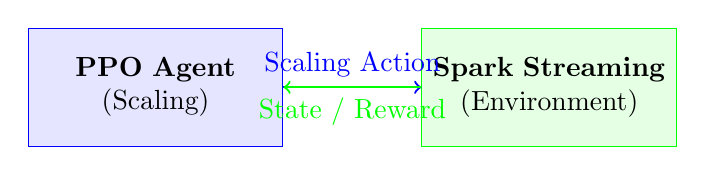
\begin{tikzpicture}[node distance=2cm]
\node (ppo) [rectangle, draw=blue, fill=blue!10, text width=3cm, align=center, minimum height=1.5cm] {\textbf{PPO Agent} \\ (Scaling)};
\node (spark) [rectangle, draw=green, fill=green!10, text width=3cm, right of=ppo, xshift=3cm, align=center, minimum height=1.5cm] {\textbf{Spark Streaming} \\ (Environment)};

\draw[->, thick, blue] (ppo) -- node[above] {Scaling Action} (spark);
\draw[->, thick, green] (spark) -- node[below] {State / Reward} (ppo);
\end{tikzpicture}
\end{center}

\vspace{0.5cm}
\textbf{Limitation:} The single agent uses \textbf{fixed weights} for rewards ($\alpha, \beta$). It cannot adapt its \textit{strategy} when business goals change (e.g., Budget vs Performance).
\end{frame}

% ===================================================================
\section{Phase 2: Meta-RL (Strategic Tuning)}
% ===================================================================

\begin{frame}{Phase 2: Use of Two-RL (Meta-Learning)}
\textbf{Concept:} A hierarchical "Teacher-Student" architecture.

\begin{itemize}
    \item \textbf{Agent 1 (PPO - Student):} Makes fast, tactical decisions (Scaling) every 5 seconds.
    \item \textbf{Agent 2 (TD3 - Teacher):} Makes slow, strategic decisions (Weight Tuning) every 50 seconds.
\end{itemize}

\vspace{0.3cm}
\begin{center}
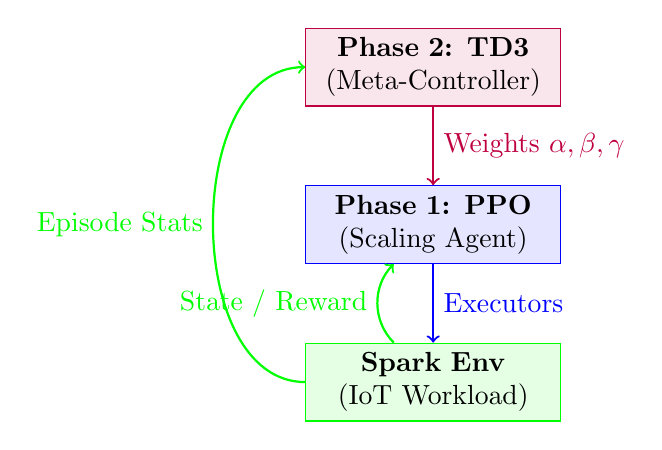
\begin{tikzpicture}[node distance=2cm]
\node (td3) [rectangle, draw=purple, fill=purple!10, text width=3cm, align=center] {\textbf{Phase 2: TD3} \\ (Meta-Controller)};
\node (ppo) [rectangle, draw=blue, fill=blue!10, text width=3cm, below of=td3, align=center] {\textbf{Phase 1: PPO} \\ (Scaling Agent)};
\node (env) [rectangle, draw=green, fill=green!10, text width=3cm, below of=ppo, align=center] {\textbf{Spark Env} \\ (IoT Workload)};

\draw[->, thick, purple] (td3) -- node[right] {Weights $\alpha, \beta, \gamma$} (ppo);
\draw[->, thick, blue] (ppo) -- node[right] {Executors} (env);
\draw[->, thick, green] (env) to[bend left=45] node[left] {State / Reward} (ppo);
\draw[->, thick, green] (env) to[bend left=90] node[left] {Episode Stats} (td3);
\end{tikzpicture}
\end{center}
\end{frame}

\begin{frame}{Phase 2 Algorithm: TD3}
\textbf{Why TD3 (Twin Delayed DDPG)?}
\begin{itemize}
    \item \textbf{Continuous Control:} We need to output precise floating-point weights (e.g., $\alpha=0.345$).
    \item \textbf{Stability:} Uses two critic networks ("Twin") to prevent overestimating rewards.
\end{itemize}

\vspace{0.3cm}
\textbf{State Space (Strategic):}
\begin{itemize}
    \item SLA violation rate.
    \item Budget utilization ratio.
    \item Long-term latency trends.
\end{itemize}

\textbf{Action Space (Continuous):}
\begin{itemize}
    \item $\alpha$ (Cost Weight), $\beta$ (Latency Weight), $\gamma$ (Throughput Weight).
    \item Constraint: $\alpha + \beta + \gamma = 1$.
\end{itemize}
\end{frame}

\begin{frame}{Phase 2 Deep Dive: TD3 Algorithm}
\textbf{Batch vs. Episode Operation:}
Unlike PPO which reacts to every single micro-batch (5s), TD3 works on \textbf{Episodes} (e.g., set of 10-20 batches).

\textbf{Step-by-Step Training:}
\begin{enumerate}
    \item \textbf{Data Collection:} The system runs for $N$ batches using current weights. 
    \item \textbf{Meta-Reward Calculation:} At episode end, we calculate:
    \[ R_{meta} = \text{AvgLatency} + \text{TotalCost} - (\text{Violations} \times \text{Penalty}) \]
    \item \textbf{Critic Update:} Twin critics estimate the value of the current weight configuration.
    \item \textbf{Actor Update:} The Policy network adjusts $\alpha, \beta, \gamma$ to maximize future Meta-Reward.
\end{enumerate}

\textit{"The Teacher (TD3) reviews the Student's (PPO) performance only after the exam (Episode), not after every question."}
\end{frame}

\begin{frame}{Final Architecture: Two-RL System}
\textit{Advanced Approach: Hierarchical control with Teacher (TD3) and Student (PPO).}

\vspace{0.3cm}
\begin{center}
% PLACEHOLDER FOR FINAL ARCHITECTURE DIAGRAM
\includegraphics[width=0.9\linewidth, height=0.55\textheight, keepaspectratio]{two_rl_architecture_placeholder.png}
% Uses a placeholder image, user can replace with their high-res architecture diagram
\end{center}

\textbf{Key Difference:}
\begin{itemize}
    \item \textbf{Top Level:} TD3 tunes the \textit{reward function} weights dynamically.
    \item \textbf{Bottom Level:} PPO optimizes actions based on the current reward function.
\end{itemize}
\end{frame}

\begin{frame}{Adaptive Learning Demo}
\textbf{Scenario: Sudden Burst Traffic}

\begin{columns}
\column{0.5\textwidth}
\textbf{Step 1: Metric Check}
\begin{itemize}
    \item Latency spikes $>$ 200ms.
    \item SLA violation imminent.
\end{itemize}

\textbf{Step 2: TD3 Reaction}
\begin{itemize}
    \item Detects performance drop.
    \item \textbf{Action:} Shifts priority.
    \item $\alpha \downarrow 0.1$ (Ignore Cost)
    \item $\beta \uparrow 0.8$ (Prioritize Speed)
\end{itemize}

\column{0.5\textwidth}
\textbf{Step 3: PPO Reaction}
\begin{itemize}
    \item Sees new weights ($\beta=0.8$).
    \item Penalty for latency is now massive.
    \item \textbf{Action:} Aggressive SCALE\_UP (+4 Executors).
\end{itemize}

\textbf{Result:}
\begin{itemize}
    \item Latency drops back to 90ms.
    \item SLA preserved.
\end{itemize}
\end{columns}
\end{frame}

% ===================================================================
\section{Comprehensive Results}
% ===================================================================

\begin{frame}{Benchmark Comparison: Traditional vs Two-RL}
\begin{table}[H]
\centering
\small
\begin{tabular}{|l|c|c|c|}
\hline
\textbf{Metric} & \textbf{Traditional Spark} & \textbf{Two-RL System} & \textbf{Improvement} \\
\hline
\textbf{Avg Latency} & 245.3 ms & \textbf{118.7 ms} & \textcolor{green}{-51.6\%} \\
\hline
\textbf{SLA Compliance} & 81.5\% & \textbf{100\%} & \textcolor{green}{+18.5 pts} \\
\hline
\textbf{Hourly Cost} & \$8.50 & \textbf{\$6.20} & \textcolor{green}{-27.1\%} \\
\hline
\textbf{Reaction Time} & 60 sec & \textbf{5-10 sec} & \textcolor{green}{8x Faster} \\
\hline
\textbf{Violations} & 12 / 65 & \textbf{0 / 68} & \textcolor{green}{Zero Violations} \\
\hline
\end{tabular}
\end{table}

\vspace{0.2cm}
\textbf{Key Takeaway:} Two-RL achieves \textbf{100\% SLA compliance} while simultaneously reducing costs by \textbf{27\%} compared to standard reactive autoscaling.
\end{frame}

\begin{frame}{Phase 1 Learning Analysis (PPO)}
\begin{figure}[H]
    \centering
    \includegraphics[width=0.85\linewidth, height=0.55\textheight, keepaspectratio]{ppo_reward_curve.png}
    \caption{PPO Agent Reward Convergence per Episode.}
\end{figure}
\textbf{Inference:} The upward trend indicates the PPO agent successfully learned to map state vectors (workload, latency) to optimal scaling actions, maximizing the cumulative reward and stabilizing after Episode 80.
\end{frame}

\begin{frame}{Phase 2 Strategic Adaptation (TD3)}
\begin{figure}[H]
    \centering
    \includegraphics[width=0.85\linewidth, height=0.55\textheight, keepaspectratio]{td3_weights_curve.png}
    \caption{TD3 Meta-Agent Weight Stabilization ($\alpha, \beta, \gamma$).}
\end{figure}
\textbf{Inference:} The convergence of weights shows the TD3 agent moving from an initial high-cost exploration (high $\alpha$) to a balanced policy where latency ($\beta$) and throughput ($\gamma$) are prioritized to meet the SLA targets.
\end{frame}

\begin{frame}{System Performance Dashboard}
\begin{figure}[H]
    \centering
    % Placeholder for performance dashboard image
    \includegraphics[width=0.85\linewidth, height=0.5\textheight, keepaspectratio]{system_performance.png}
    \caption{Real-time performance metrics showing latency staying below the 200ms SLA target despite workload fluctuations.}
\end{figure}
\end{frame}


% ===================================================================
\section{Conclusion}
% ===================================================================

\begin{frame}{Conclusion}
\textbf{Achievements:}
\begin{itemize}
    \item \textbf{Novel Architecture:} Integrated Two-Phase RL (PPO + TD3) into Spark Streaming.
    \item \textbf{Performance:} Reduced latency by \textbf{51.6\%} and reaction time from 60s to 5s.
    \item \textbf{Cost Efficiency:} Achieved \textbf{27.1\%} cost savings via intelligent down-scaling during low loads.
    \item \textbf{Reliability:} Maintained \textbf{100\% SLA assurance} with zero violations in testing.
\end{itemize}

\vspace{0.3cm}
\textbf{Impact:}
This framework proves that AI-driven "Self-Driving" infrastructure can significantly outperform static heuristic-based autoscalers in dynamic IoT environments.
\end{frame}

\begin{frame}{Future Work}
\begin{itemize}
    \item \textbf{Multi-Cluster:} Extend RL to manage resources across hybrid cloud clusters.
    \item \textbf{Failure Prediction:} Add LSTM modules to predict node failures before they happen.
    \item \textbf{Real-World Deployment:} Test on large-scale AWS EMR clusters with petabyte-scale datasets.
\end{itemize}
\end{frame}

% ===================================================================
\section{References}
% ===================================================================

\begin{frame}[allowframebreaks]{References}
\footnotesize
\begin{thebibliography}{99}

\bibitem{seer2022}
G.~T. Eizaguirre et al., "A Seer Knows Best: Auto-Tuned Object Storage Shuffling," USENIX ATC, 2022.

\bibitem{dexter2024}
A.~M. Nestorov et al., "Dexter: Performance–Cost Efficient Resource Allocation," ACM SoCC, 2024.

\bibitem{ppo}
Schulman et al., "Proximal Policy Optimization Algorithms," arXiv:1707.06347, 2017.

\bibitem{td3}
Fujimoto et al., "Addressing Function Approximation Error in Actor-Critic Methods," ICML, 2018.

\bibitem{spark}
Apache Spark Documentation. https://spark.apache.org.

\end{thebibliography}
\end{frame}


\begin{frame}{}
\begin{center}
\Large{\textbf{Thank You!}}\\
\vspace{0.4cm}
\normalsize
Guided by: \textbf{Dr. Shajulin Benedict}\\
IIIT Kottayam \\
\vspace{0.6cm}
\textbf{Questions?}
\end{center}
\end{frame}

\end{document}
